\documentclass{ltjsarticle}
\usepackage{amsmath}
\usepackage{amssymb}
\usepackage{ascmac}
\usepackage[dvipdfmx]{graphicx}
\usepackage[colorlinks=true, allcolors=blue]{hyperref}
\usepackage{fancybox}
\usepackage{tikz}
\usepackage{subcaption}
\usetikzlibrary{shapes,arrows}

\begin{document}

\title{深層学習 Day1}
\author{秋葉洋哉}
\maketitle

\section{ニューラルネットワーク}
\subsection{識別モデルと生成モデル}
識別モデルとは、データを目的のクラスに分類するための方法である。一方で、生成モデルとは、特定のクラスのデータを生成するための方法である。例えば、犬という画像を入力で与えた場合にそれが犬である確率を出力するのが識別モデルであり、犬というクラスを与えた場合に犬の画像を生成するのが生成モデルである。
\par
識別モデルは、基本的に高次元(=データ量の多いもの)から低次元(=データ量の少ないもの)へと変換することに長けており、画像認識等で用いられる。一方で、生成モデルでは、低次元から高次元へと変換することに長けており、画像の生成等で用いられる。
\par
識別モデルでは、決定木・ロジスティック回帰・SVM・ニューラルネットワークなどがある。生成モデルでは、隠れマルコフモデル・ベイジアンネットワーク・変分オートエンコーダー(VAE)・敵対的生成ネットワーク(GAN)などがある。
\par
生成モデルは、ベイズの定理を用いて識別器を作成する方法である。
入力が生まれる確率と、クラスが生まれる確率を与え、それを用いてクラスを推定する。つまり、
\begin{align}
  P(x|C_k)P(C_k)
\end{align}
によって各クラスの生起確率を求め、最大のクラスを選択するというものである。
生成モデルではデータを人工的に生成できることが特徴である。
ベイズの定理は、
\begin{align}
  P(C_k|x) = \frac{P(x|C_k)P(C_k)}{P(x)}
\end{align}
で表される。

\subsection{万能近似定理}
万能近似定理とは、任意の連続関数をニューラルネットワークで近似できるという定理である。この定理により、ニューラルネットワークは、非常に高い表現力を持つことがわかる。この定理により、ニューラルネットワークは、多くの分野で利用されている。

\subsection{ニューラルネットワークの概要}
ニューラルネットワークは、脳の神経細胞を模倣したモデルである。ニューラルネットワークは、入力層・中間層・出力層から構成される。入力層は、入力データを受け取る層であり、中間層は、入力データを変換する層であり、出力層は、データを出力する層である。多層パーセプトロン(MLP)・畳み込みニューラルネットワーク(CNN)・再帰型ニューラルネットワーク(RNN)といった種類を有する。

\begin{itembox}[l]{確認テスト}
Q: ディープラーニングは、結局なにをやろうとしているか2行以内で述べよ。また、最適化する値は何か。

A: ディープラーニングは、多層のニューラルネットワークを用いて、高度な特徴を抽出し、複雑な問題を解決することを目的としている。最適化する値は、誤差関数を最小化する重み$w$とバイアス$b$である。

Q: 入力層2ノード1層・中間層3ノード2層・出力層1ノード1層のネットワークを書け。

A: 図\ref{fig:2-3-1}を参照。

\end{itembox}

\begin{figure}[htbp]
  \centering
  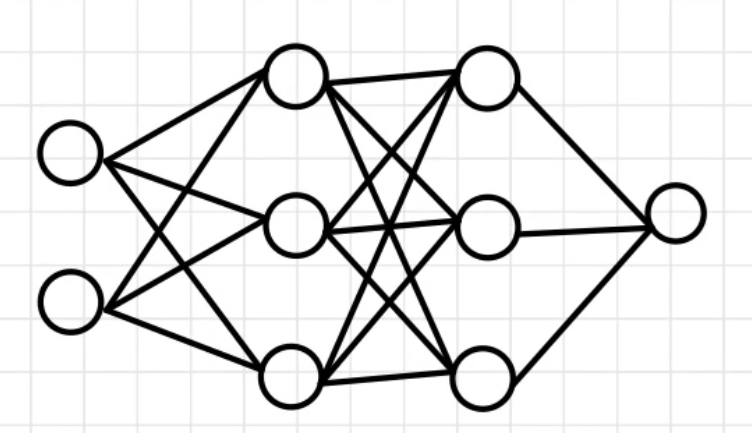
\includegraphics[width=8cm]{./capture/confirm_test/day1_01_1.png}
  \caption{入力層2ノード1層・中間層3ノード2層・出力層1ノード1層のネットワーク}
  \label{fig:2-3-1}
\end{figure}

\par
ニューラルネットワークは、自動売買・チャットボット・画像認識・音声認識・自然言語処理・囲碁将棋AIなど、多くの分野で利用されている。
\par
ニューラルネットワークの1つのノードに対して、入力$x_i$, 重み$w_i$, バイアス$b$, 総入力$u$, 出力$z$, 活性化関数$f$とすると、
\begin{align}
  u &= \sum_{i=1}^{n}w_ix_i + b \\
  z &= f(u)
\end{align}
で表される。この出力は次のノードの入力として用いられることになる。
\begin{itembox}[l]{確認テスト}
  Q: 図\ref{fig:day1_02_1}に動物分類の実例を入れろ。

  A: 図\ref{fig:day1_02_2}を参照

  Q: 図\ref{fig:day1_02_3}の数式を書け。

  A: 図\ref{fig:day1_02_4}を参照
\end{itembox}
\begin{figure}[ht]
    \centering
    \begin{subfigure}[b]{0.45\textwidth}
      \centering
      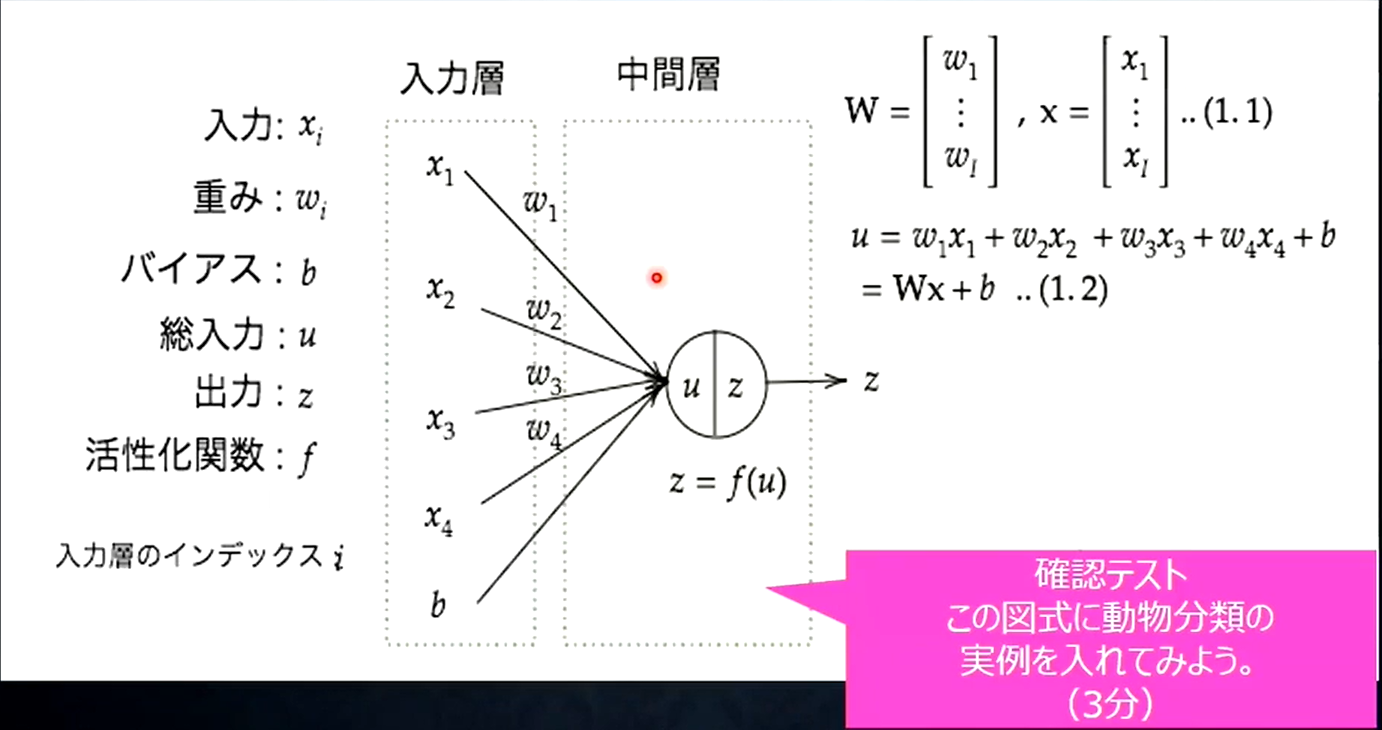
\includegraphics[width=\textwidth]{./capture/confirm_test/day1_02_1.png}
      \caption{}
      \label{fig:day1_02_1}
    \end{subfigure}
    \hfill
    \begin{subfigure}[b]{0.45\textwidth}
      \centering
      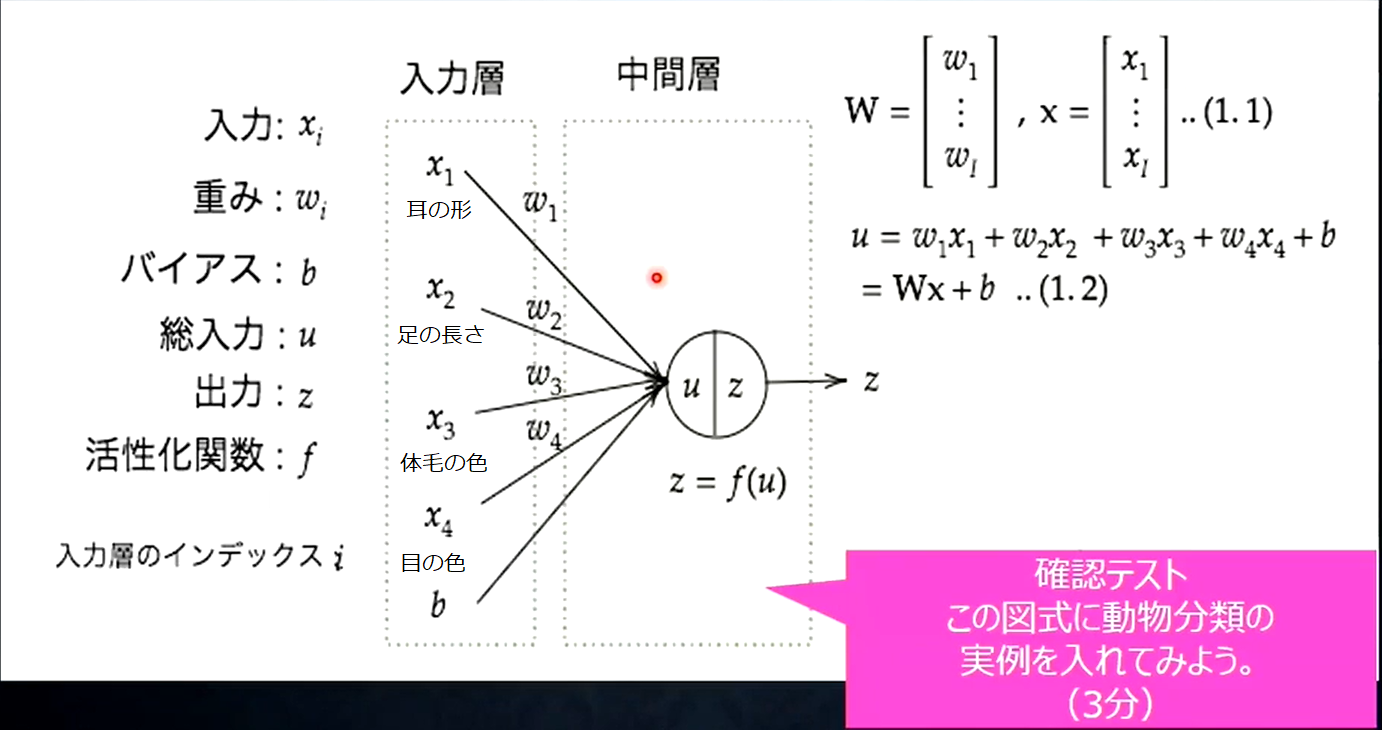
\includegraphics[width=\textwidth]{./capture/confirm_test/day1_02_2.png}
      \caption{}
      \label{fig:day1_02_2}
    \end{subfigure}
    \caption{}
\end{figure}

\begin{figure}[ht]
  \centering
  \begin{subfigure}[b]{0.45\textwidth}
    \centering
    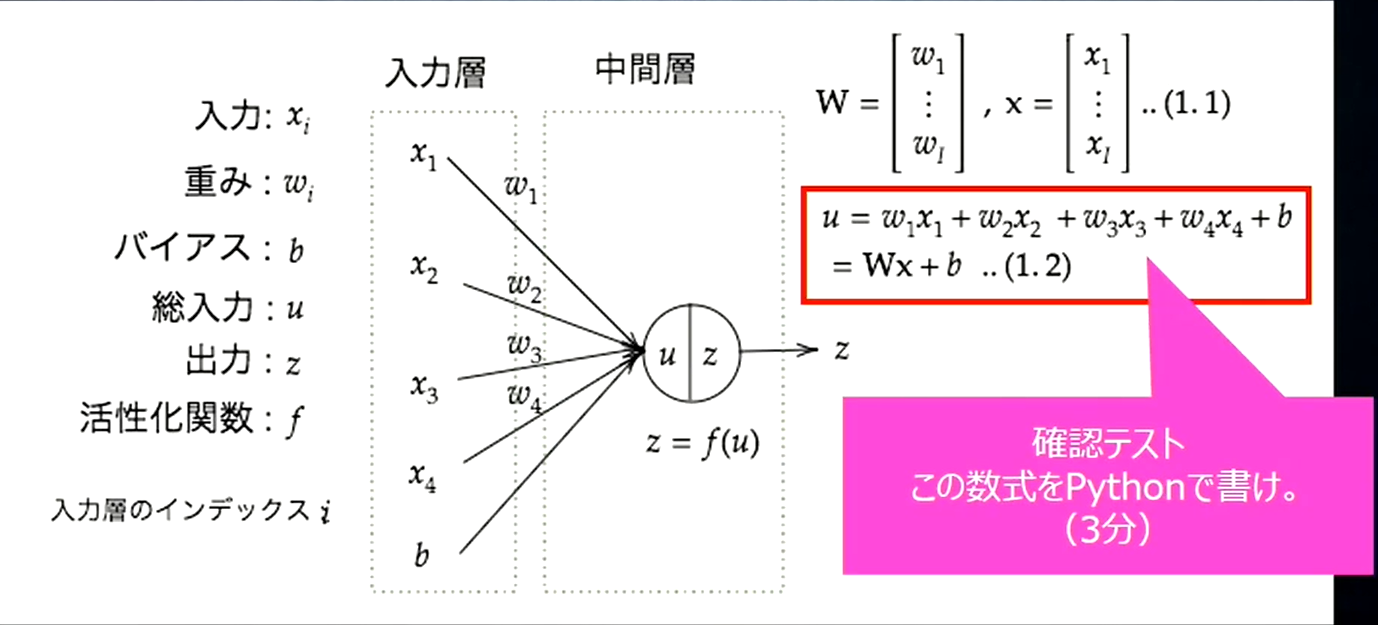
\includegraphics[width=\textwidth]{./capture/confirm_test/day1_02_3.png}
    \caption{}
    \label{fig:day1_02_3}
  \end{subfigure}
  \hfill
  \begin{subfigure}[b]{0.45\textwidth}
    \centering
    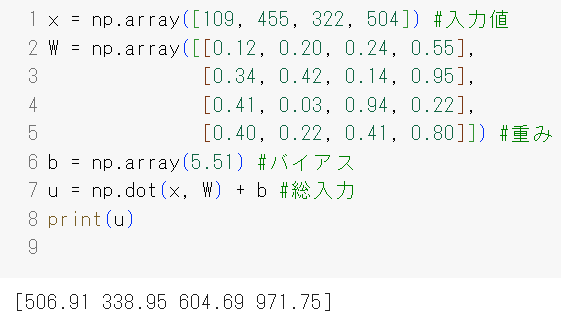
\includegraphics[width=\textwidth]{./capture/confirm_test/day1_02_4.png}
    \caption{}
    \label{fig:day1_02_4}
  \end{subfigure}
  \caption{}
\end{figure}

中間層と出力層で用いられる活性化関数に違いがある。
中間層では、ReLU関数、シグモイド関数、ステップ関数といった関数が用いられることが多い。
出力層では、ソフトマックス関数(多値分類)、シグモイド関数(二値分類)、恒等関数(回帰)といった関数が用いられることが多い。
出力層において用いる活性化関数と誤差関数は、扱う問題に応じて選択する必要がある。
\begin{enumerate}
  \item 回帰問題の場合 → 恒等関数・二乗和誤差
  \item 2値分類問題の場合 → シグモイド関数・交差エントロピー誤差
  \item 多クラス分類問題の場合 → ソフトマックス関数・交差エントロピー誤差
\end{enumerate}

\subsection{活性化関数}
活性化関数とは、入力を出力に変換する関数である。活性化関数には、ステップ関数・シグモイド関数・ReLU関数・恒等関数・ソフトマックス関数などがある。
\subsubsection{ステップ関数}
閾値を超えたら発火する関数で、0か1を示す。
Pythonのサンプルコードを示す。
\begin{screen}
  \begin{verbatim}
    def step_function(x):
        if x > 0:
            return 1
        else:
            return 0
  \end{verbatim}
\end{screen}

\subsubsection{シグモイド関数}
勾配消失問題がある関数で、0から1の値を示す。
Pythonのサンプルコードを示す。
\begin{screen}
  \begin{verbatim}
    def sigmoid(x):
        return 1 / (1 + np.exp(-x))
  \end{verbatim}
\end{screen}


\subsubsection{ReLU関数}
勾配消失問題を回避し、スパース化によって過学習を防ぐ関数である。
Pythonのサンプルコードを示す。
\begin{screen}
  \begin{verbatim}
    def relu(x):
        return np.maximum(0, x)
  \end{verbatim}
\end{screen}


\subsubsection{恒等関数}
入力をそのまま出力する関数である。
Pythonのサンプルコードを示す。
\begin{screen}
  \begin{verbatim}
    def identity_function(x):
        return x
  \end{verbatim}
\end{screen}

\begin{itembox}[l]{確認テスト}
  Q: 図\ref{fig:day1_03_1}の赤枠に該当する箇所をソースコードから抜き出せ。

  A: 図\ref{fig:day1_03_2}を参照
\end{itembox}

\begin{figure}[ht]
  \centering
  \begin{subfigure}[b]{0.45\textwidth}
    \centering
    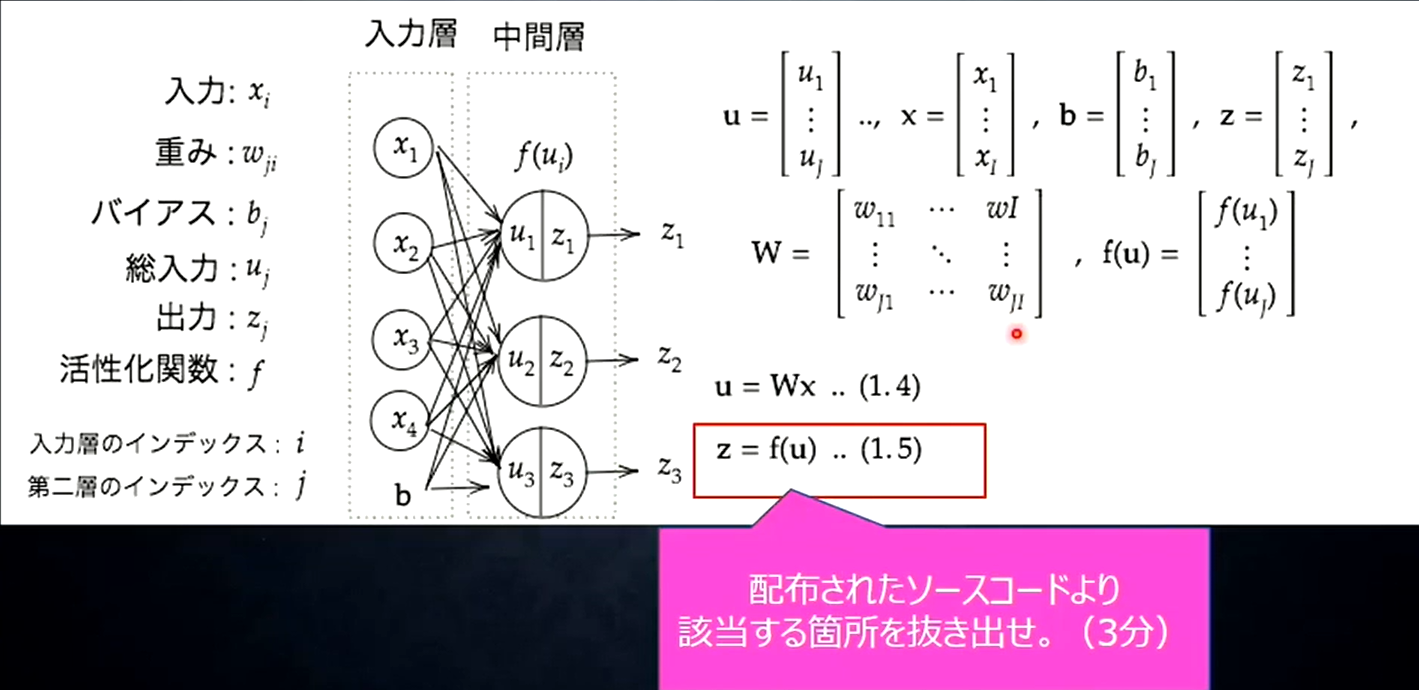
\includegraphics[width=\textwidth]{./capture/confirm_test/day1_03_1.png}
    \caption{}
    \label{fig:day1_03_1}
  \end{subfigure}
  \hfill
  \begin{subfigure}[b]{0.45\textwidth}
    \centering
    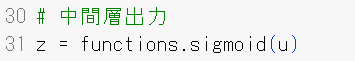
\includegraphics[width=\textwidth]{./capture/confirm_test/day1_03_2.png}
    \caption{}
    \label{fig:day1_03_2}
  \end{subfigure}
  \caption{}
\end{figure}

\subsubsection{ソフトマックス関数}
出力の総和が1になる関数である。
数式で表すと、以下の通りとなる。
\begin{align}
  f(i,u) = \frac{\exp(u_i)}{\sum_{k=1}^{K}\exp(u_k)}
\end{align}
Pythonのサンプルコードを示す。
\begin{screen}
  \begin{verbatim}
    def softmax(x):
        return np.exp(x) / np.sum(np.exp(x))
  \end{verbatim}
\end{screen}

\begin{itembox}[l]{確認テスト}
  Q: 図\ref{fig:day1_05_1}の丸1から丸3までの数式に該当するソースコードを示し、1行ずつ処理の説明をせよ。

  A: 図\ref{fig:day1_05_2}を参照。それぞれの説明は以下の通り。
  \begin{itemize}
    \item[①.] 2層目の総出力$u_2$を入力として、ソフトマックス関数を適用する。
    \item[②.] ソフトマックス関数の分子を計算する。
    \item[③.] ソフトマックス関数の分母を計算する。
  \end{itemize}
  
\end{itembox}

\begin{figure}[ht]
  \centering
  \begin{subfigure}[b]{0.45\textwidth}
    \centering
    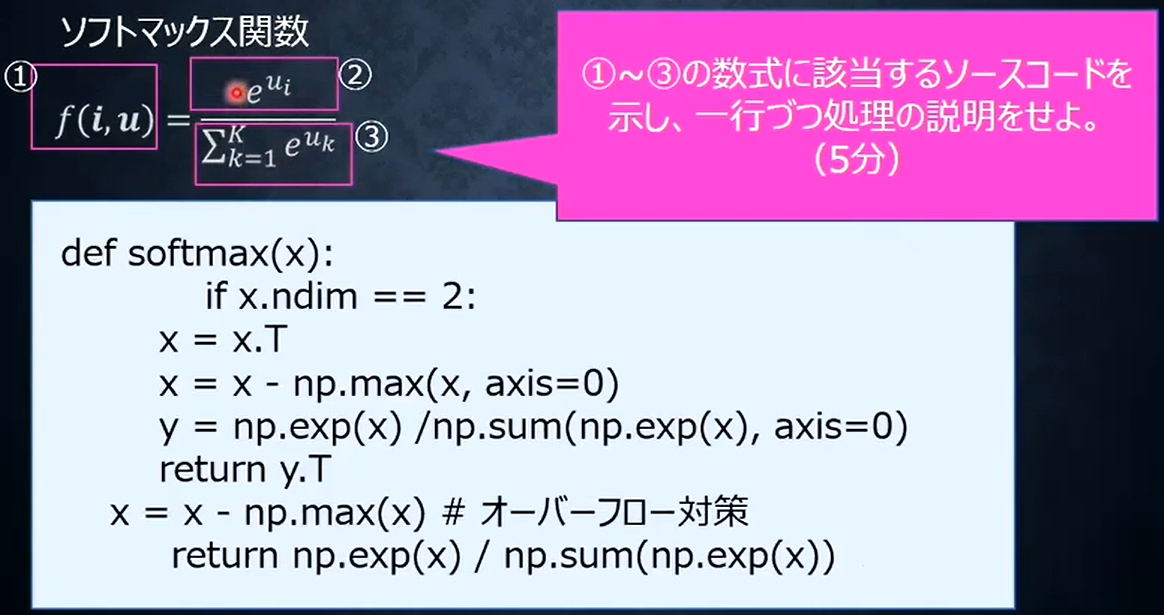
\includegraphics[width=\textwidth]{./capture/confirm_test/day1_05_1.png}
    \caption{}
    \label{fig:day1_05_1}
  \end{subfigure}
  \hfill
  \begin{subfigure}[b]{0.45\textwidth}
    \centering
    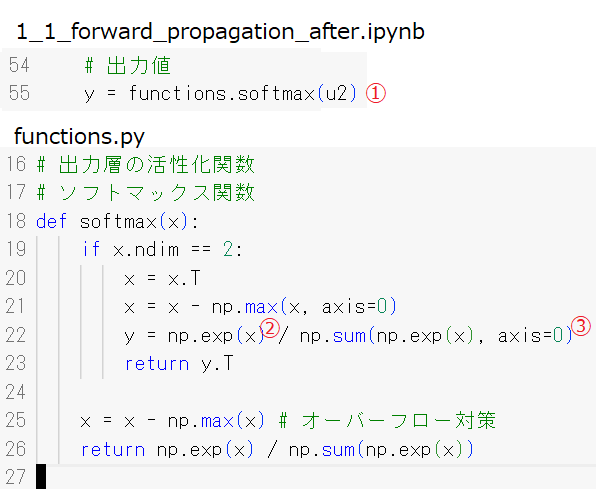
\includegraphics[width=\textwidth]{./capture/confirm_test/day1_05_2.png}
    \caption{}
    \label{fig:day1_05_2}
  \end{subfigure}
  \caption{}
\end{figure}

\subsection{誤差関数}
\subsubsection{二乗和誤差}
二乗和誤差とは、予測値と正解値の差の2乗和を2で割ったものである。
数式で表すと、以下の通りとなる。
\begin{align}
  E(\mathbf{w}) = \frac{1}{2}\sum_{i=1}^{w}(y_i - t_i)^2
\end{align}

\begin{itembox}[l]{確認テスト}
  Q: 二乗和誤差は、なぜ単なる引き算ではなく二乗するのか述べよ。
  
  A: 二乗和誤差は、予測値と正解値の差を取ることで、正解値との誤差を表す。二乗することで、正解値との誤差が大きい場合に誤差が大きくなり、正解値との誤差が小さい場合に誤差が小さくなるようにするためである。

  Q : 二乗和誤差の$\frac{1}{2}$はどういう意味を持つか述べよ。

  A: $\sum_{i=1}^{w} (y_i-t_i)^2$の微分値は以下の通りである。
  \begin{align}
    \frac{\partial E}{\partial y_i} &= \frac{\partial}{\partial y_i}\left( \sum_{i=1}^{n}(y_i - t_i)^2 \right) \\
    &= 2(y_i - t_i)
  \end{align}
  二乗和誤差の定義式で$\frac{1}{2}$を掛けるのは、前に出た2を消し、微分値を$(y_i - t_i)$として、計算を簡単にするためである。
\end{itembox}

\begin{itembox}{平均二乗和誤差と二乗和誤差}
機械学習でよく用いられる平均二乗誤差(Mean Squared Error: MSE)は、二乗和誤差の分母2をデータ数に変えて計算したものである。数式で表すと、以下の通りとなる。
\begin{align}
  E(\mathbf{w}) = \frac{1}{n}\sum_{i=1}^{w}(y_i - t_i)^2
\end{align}
平均二乗和誤差は、データ数によって誤差のスケールが変わるため、データ数が異なる場合でも誤差を比較することができる。
一方で、二乗和誤差は、データ数によって誤差のスケールが変わらないため、データ数が異なる場合は誤差を比較することができないが、計算が簡単という特徴がある。
\end{itembox}

\subsubsection{交差エントロピー誤差}
交差エントロピー誤差とは、2つの確率分布の違いを表す指標である。
数式で表すと、以下の通りとなる。
\begin{align}
  E(\mathbf{w}) = -\sum_{i=1}^{w} t_i log(y_i)
\end{align}
ただし、$t_i$は正解ラベル、$y_i$は予測値を表す。
この式を例を示しながら説明する。
写真に写っている動物が犬であるとする。
分類器は、犬・猫・ネズミを見分けることができるとし、いずれかのクラスの確率を出力する。
今、犬・猫・ネズミのそれぞれの確率を0.8, 0.1, 0.1であると予測した場合、交差エントロピー誤差は、
\begin{align}
  E &= -1.0*\log(0.8) - 0.0*\log(0.1) - 0.0*\log(0.1) \\
   &= 0.223
\end{align}
となる。次に、犬・猫・ネズミのそれぞれの確率を0.4, 0.3, 0.3 であると予測した場合、交差エントロピー誤差は、
\begin{align}
  E &= -1.0*\log(0.4) - 0.0*\log(0.3) - 0.0*\log(0.3) \\
   &= 0.52
\end{align}
となる。このように、交差エントロピー誤差は、予測が正解に近いほど小さくなり、予測が不正解に近いほど大きくなる。これは直観的にも誤差関数として交差エントロピー誤差が適していることが分かる。

\begin{itembox}[l]{確認テスト}
  Q: 図\ref{fig:day1_05_3}の丸1から丸2までの数式に該当するソースコードを示し、1行ずつ処理の説明をせよ。

  A: 図\ref{fig:day1_05_4}を参照。それぞれの説明は以下の通り。
  \begin{itemize}
    \item[①.] 正解値$d$, 予測値$y$を入力を与えて、交差エントロピー誤差を呼び出す。 
    \item[②.] $\log{y^d} = d\log{y}$として、numpyのlog関数を用いて計算する。1.0d-7を加えるのは、log(0)を防ぐためである。
  \end{itemize}
  
\end{itembox}

\begin{figure}[ht]
  \centering
  \begin{subfigure}[b]{0.45\textwidth}
    \centering
    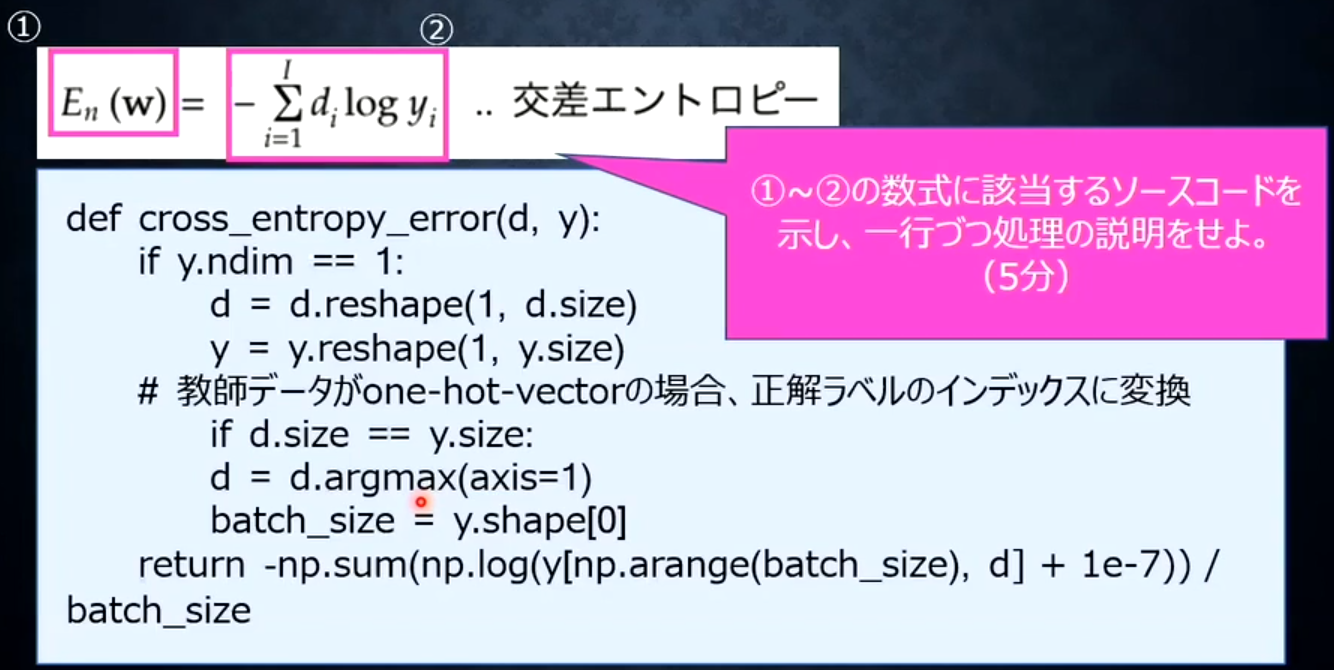
\includegraphics[width=\textwidth]{./capture/confirm_test/day1_05_3.png}
    \caption{}
    \label{fig:day1_05_3}
  \end{subfigure}
  \hfill
  \begin{subfigure}[b]{0.45\textwidth}
    \centering
    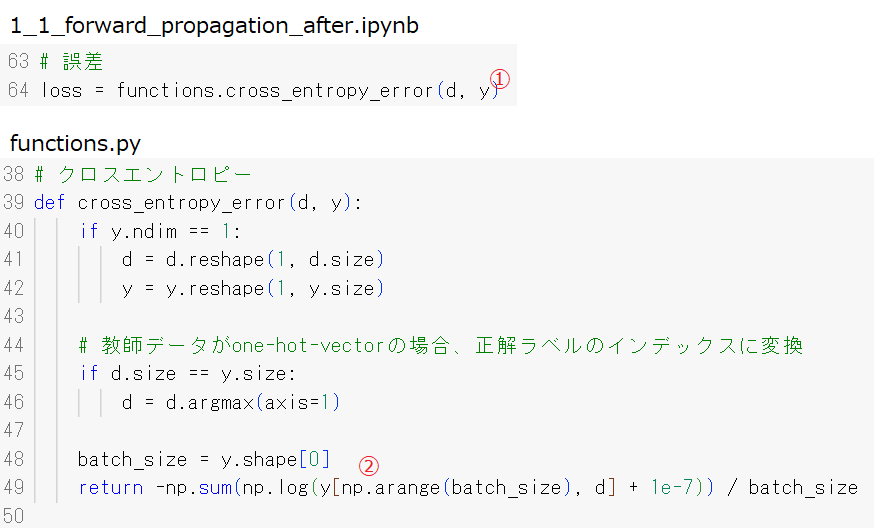
\includegraphics[width=\textwidth]{./capture/confirm_test/day1_05_4.png}
    \caption{}
    \label{fig:day1_05_4}
  \end{subfigure}
  \caption{}
\end{figure}

\subsubsection{カテゴリカル交差エントロピー誤差}
カテゴリカル交差エントロピー誤差とは、多クラス分類問題において用いられる誤差関数である。
数式で表すと、以下の通りとなる。
\begin{align}
  E= -\sum_{j=1}^{L-1} \sum_{i=1}^{M-1} t_{ji} \log(y_{ji})
\end{align}
ただし、$t_i$は正解ラベル、$y_i$は予測値、$L$はクラス数、$M$はクラス数を表す。
交差エントロピー誤差をクラス間で拡張し、すべてを足し合わせている。


\subsection{勾配降下法}
勾配降下法とは、導関数を用いて数値的に方程式の解を求めるための方法である。
深層学習では、学習を通して誤差関数を最小にするパラメータ$\mathbf{w}$を求めることが目的であり、勾配降下法はそのための手法の一つとして用いられる。
勾配降下法は、以下の手順で行われる。
\begin{enumerate}
  \item パラメータ$\mathbf{w}$を初期化する
  \item 誤差関数$E(\mathbf{w})$を最小化するために、$\mathbf{w}$を更新する
  \item 収束するまで2を繰り返す
\end{enumerate}
数式で表すと、以下の通りとなる。
\begin{align}
  \label{eq:gradient_descent}
  \mathbf{w}^{(t+1)} = \mathbf{w}^{(t)} - \epsilon E(\mathbf{w})
\end{align}
ここで、$\epsilon$は学習率を表す。
学習率は、パラメータの更新量を調整するためのハイパーパラメータであり、大きすぎると発散し、小さすぎると収束が遅くなるため、適切な値を設定する必要がある。
勾配降下法には様々な種類があり、Momentum・AdaGrad・Adadelta・Adamなどがある。
\begin{itembox}[l]{確認テスト}
  Q: 式\eqref{eq:gradient_descent}に該当するソースコードを示せ。

  A: 図\ref{fig:day1_06_1}を参照
\end{itembox}

\begin{figure}[ht]
  \centering
  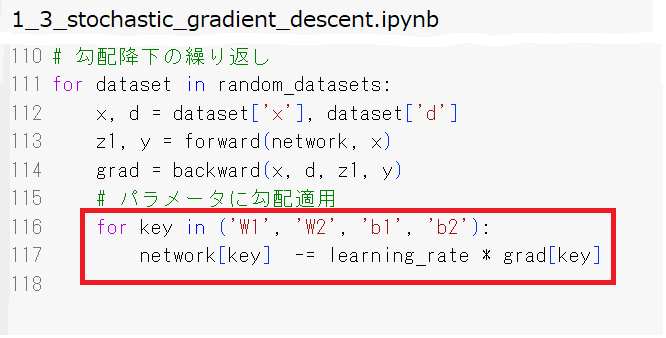
\includegraphics[width=10cm]{./capture/confirm_test/day1_06_1.png}
  \caption{}
  \label{fig:day1_06_1}
\end{figure}

\subsection{確率的勾配降下法(SGD)}
確率的勾配降下法とは、勾配降下法の一種であり、毎回違う学習データをランダムに選んで行う方法である。
計算コストを下げたり、局所解に陥ることを防ぐために用いられる。
勾配降下法を用いた深層学習モデルの学習データの選び方は、
\begin{enumerate}
  \item バッチ学習
  \item ミニバッチ学習
  \item オンライン学習
\end{enumerate}
の3つが挙げられる。
\par
バッチ学習は、エポック毎に全てのデータを使って傾きを逐次求め、最適解を見つける方法である。学習結果が安定しやすいという特徴を持つ。新たな訓練データが追加された場合に、再度全データを用いて計算を行う必要があるため、計算コストが高い。
\par
ミニバッチ学習は、すべてのデータの中から一部を取り出して学習する方法で、局所最適解を回避しやすいという特徴を持つ。バッチ学習とオンライン学習の中間の特徴を持つ。すべてのデータで学習し終えた時に1エポックが終了し、重みが更新される。
\par
オンライン学習は、すべてのデータの中から1つを取り出して学習する方法で、ミニバッチ学習よりも局所最適解を回避しやすいという特徴を持つ。計算コストが低いが、学習結果が不安定であるという特徴を持つ。
\par
深層学習のモデリングにおいては、ミニバッチ学習が最も一般的に用いられる。
その理由として、確率的勾配法のメリットを損なわずに、計算資源を有効利用することができるからである。
例えば、1000万件の学習データがあった場合、それをバッチ学習で学習しようとすると、1000万件のデータを一度に計算する必要がある。現代のコンピュータでは、1000万件のデータの計算には莫大な時間を要してしまう。そのため1000件ずつのミニバッチを作成し、それを10000回繰り返す際に、他の資源でも同時平行で計算することで時間を短縮させる。これには、CPUのスレッド並列化やGPUのSIMD並列化という技術が用いられる。

\begin{itembox}[l]{確認テスト}
  Q: $\mathbf{w^{(t+1)}} = \mathbf{w^{(t)}} - \epsilon \nabla E_t$ の数式の意味を図に書いて説明せよ。

  A: 図\ref{fig:day1_08_1}を参照
\end{itembox}

\begin{figure}[ht]
  \centering
  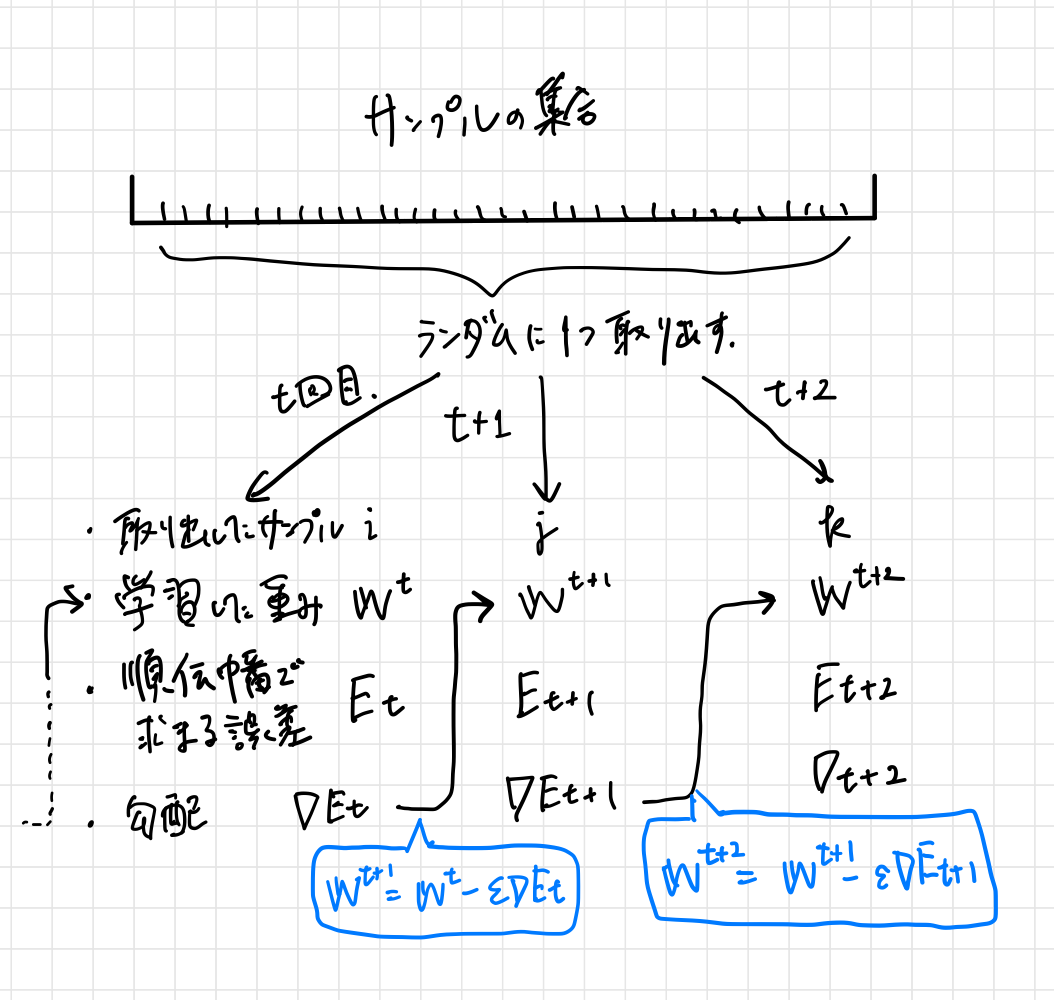
\includegraphics[width=10cm]{./capture/confirm_test/day1_08_1.png}
  \caption{}
  \label{fig:day1_08_1}
\end{figure}

\subsection{誤差逆伝播法}
勾配降下法を用いて、重みとバイアスを更新する際に用いられる方法が誤差逆伝播法である。
誤差逆伝播法は、出力層から入力層に向かって、誤差を逆伝播させることで、各層の重みとバイアスを更新する方法である。
誤差逆伝播法は、以下の手順で行われる。
\begin{enumerate}
  \item 順伝播
  \item 誤差逆伝播
  \item 重みとバイアスの更新
\end{enumerate}
数式で表すと、以下の通りとなる。
\begin{align}
  w &\leftarrow w - \epsilon \frac{\partial E}{\partial w} \\
  b &\leftarrow b - \epsilon \frac{\partial E}{\partial b}
\end{align}
ただし、$w$は重み、$b$はバイアス、$\epsilon$は学習率、$E$は誤差関数を表す。
勾配を求めることができれば、上式を用いて重みとバイアスを更新することができる。

以下では、ノード$i$における前ノード$j$との間の重み$w_{ij}$の勾配を求める。
まず、$\frac{\partial E}{\partial w_{ij}}$を求める。
\begin{align}
  \frac{\partial E}{\partial w_{ij}} = \frac{\partial E}{\partial u_i}\frac{\partial u_i}{\partial w_{ij}}
\end{align}
$u_i$は、ノード$i$の総入力を表し、
\begin{align}
  u_i = \sum_{j=1}^{m}w_{ij}y_j + b_i
\end{align}
であるから、$\frac{\partial u_i}{\partial w_{ij}}$は、
\begin{align}
  \frac{\partial u_i}{\partial w_{ij}} &= \frac{\partial}{\partial w_{ij}}\left( \sum_{j=1}^{m}w_{ij}y_j + b_i \right)\\
   &= y_j
\end{align}
となる。また、$\frac{\partial E}{\partial u_i}$は、
\begin{align}
  \frac{\partial E}{\partial u_i} = \frac{\partial E}{\partial y_i}\frac{\partial y_i}{\partial u_i}
\end{align}
で表される。ここで、$E$が二乗和誤差の場合、
\begin{align}
  \frac{\partial E}{\partial y_i} &= \frac{\partial}{\partial y_i}\left( \frac{1}{2} \left( \sum_{i=1}^{n}(y_i - t_i)^2 \right) \right) \\
  &= y_i - t_i
\end{align}
となる。また、$y_i$が恒等関数の場合、
\begin{align}
  \frac{\partial y_i}{\partial u_i} &= \frac{\partial}{\partial u_i}u_i \\
  &= 1
\end{align}
となる。以上より、$\frac{\partial E}{\partial u_i}$は、
\begin{align}
  \frac{\partial E}{\partial u_i} = (y_i - t_i) \times 1 = y_i - t_i
\end{align}
となる。よって、$\frac{\partial E}{\partial w_{ij}}$は、
\begin{align}
  \frac{\partial E}{\partial w_{ij}} = (y_i - t_i)y_j
\end{align}
となる。同様に、バイアス$b_i$についても、
\begin{align}
  \frac{\partial E}{\partial b_i} = \frac{\partial E}{\partial u_i}\frac{\partial u_i}{\partial b_i} = y_i - t_i
\end{align}
となる。以上より、重みとバイアスの更新式は、
\begin{align}
  w_{ij} &\leftarrow w_{ij} - \epsilon(y_i - t_i)y_j \\
  b_i &\leftarrow b_i - \epsilon(y_i - t_i)
\end{align}
となる。これを、ノード$i$におけるすべての前ノード$j$について計算するために、行列表現で表すと、
\begin{align}
  \mathbf{w} &\leftarrow \mathbf{w} - \epsilon \mathbf{y}^T(y_i - t_i) \\
  \mathbf{b} &\leftarrow \mathbf{b} - \epsilon(y_i - t_i)
\end{align}
となる。ここで、$\mathbf{y}$を転置しているのは、$\mathbf{w}$と形状を合わせるためである。

図\ref{fig:backprop}に、誤差逆伝播の概要を示す。
\begin{figure}[htbp]
  \centering
  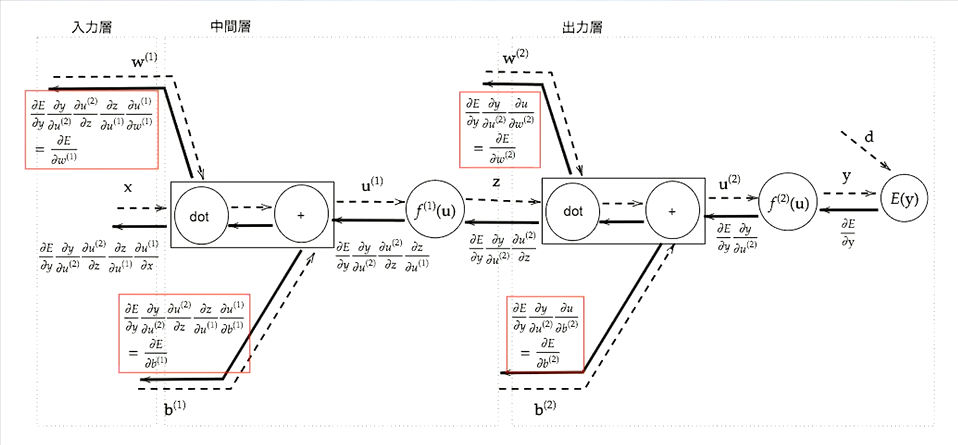
\includegraphics[width=13cm]{./capture/backprop.png}
  \caption{誤差逆伝播法における勾配}
  \label{fig:backprop}
\end{figure}

\newpage

\begin{itembox}[l]{確認テスト}
  Q: 誤差逆伝搬法では不要な再帰的処理を避けることができる。すでに行った計算結果を保持しているソースコードを抽出せよ。

  A: 図\ref{fig:day1_10_1}を参照

  Q: $\frac{\partial E}{\partial y} \frac{\partial y}{\partial u}$と、$\frac{\partial E}{\partial y} \frac{\partial y}{\partial u} \frac{\partial u}{\partial w_{ji}^{(2)}}$に該当するソースコードを探せ。

  A: 図\ref{fig:day1_10_2}を参照
\end{itembox}

\begin{figure}[ht]
  \centering
  \begin{subfigure}[b]{0.45\textwidth}
    \centering
    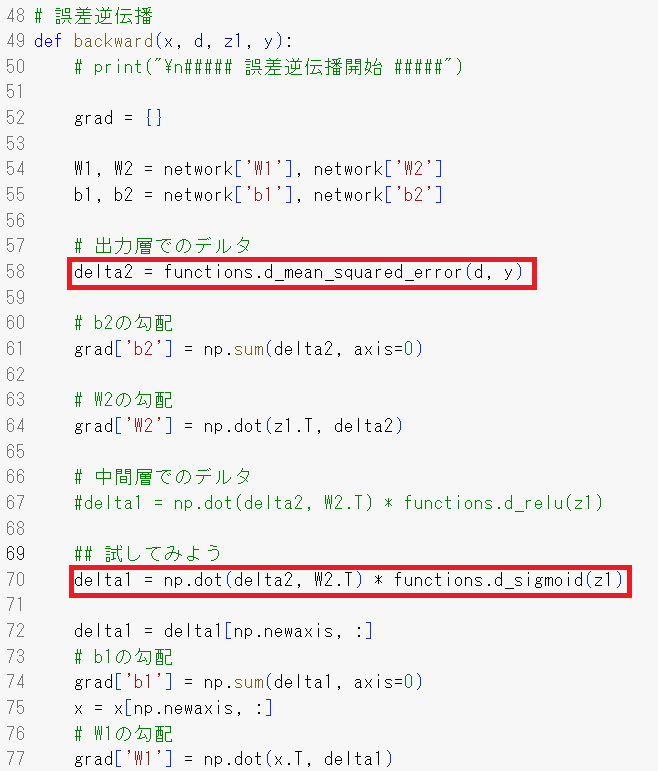
\includegraphics[width=\textwidth]{./capture/confirm_test/day1_10_1.png}
    \caption{}
    \label{fig:day1_10_1}
  \end{subfigure}
  \hfill
  \begin{subfigure}[b]{0.45\textwidth}
    \centering
    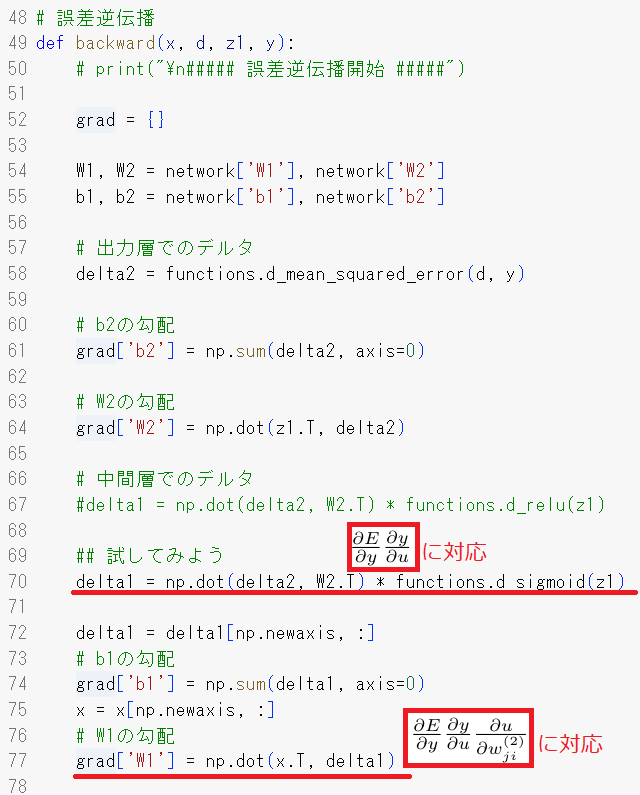
\includegraphics[width=\textwidth]{./capture/confirm_test/day1_10_2.png}
    \caption{}
    \label{fig:day1_10_2}
  \end{subfigure}
  \caption{}
\end{figure}

\newpage

\begin{itembox}[l]{計算グラフ}
  計算グラフとは計算の過程をグラフで視覚化したものである。これを用いることで、複雑な偏微分の連なりを分解し、出力へ影響を与えるノードを絞りこむことができるようになる。
  計算グラフは複数の「ノード」と「エッジ」から構成される。
  例えば、a,b,c,d,e,fをノードとし、
  \begin{align}
    e = ab\\
    f = cd\\
    g = e + f
  \end{align}
  を計算グラフで表すと、図\ref{fig:calc_graph}の青字ようになる。これは順伝播を表す。
  \par
  ここで、最終的な出力である$g$が、それぞれのノードの影響をどの程度受けるか知りたいとする。
  偏微分について以下が成立することは明白である。
  \begin{align}
    f(a,b) &= ab\\
    \frac{\partial f}{\partial a} &= b\\
    \frac{\partial f}{\partial b} &= a\\
    g(e,f) &= e + f\\
    \frac{\partial g}{\partial e} &= 1\\
    \frac{\partial g}{\partial f} &= 1
  \end{align}
  $e, f$は、値の大きさに依らずそれぞれ1の影響を$g$に与える。つまり、$e$の値が1変わったら$g$が1変わるという意味である。
  $a, b, c, d$は、$e, f$に対してそれぞれ2, 3, 5, 4の影響を与える。これらは同様に、$a, b, c, d$の値が1変わったら、$e, f$がそれぞれ2, 3, 5, 4変わるという意味である。さらに$e, f$は$g$に等倍の影響であるため、$a, b, c, d$が1変わったら、$g$が$2+3+5+4=14$変わることがわかる。これらの処理の流れは、図\ref{fig:calc_graph}の黄色で示されており、逆伝播を表す。
  \par
  ここでは、計算グラフを用いることで、$g$に与える影響が最も大きいノードは$c$であることが分かった。

\end{itembox}

\begin{figure}[htbp]
  \centering
  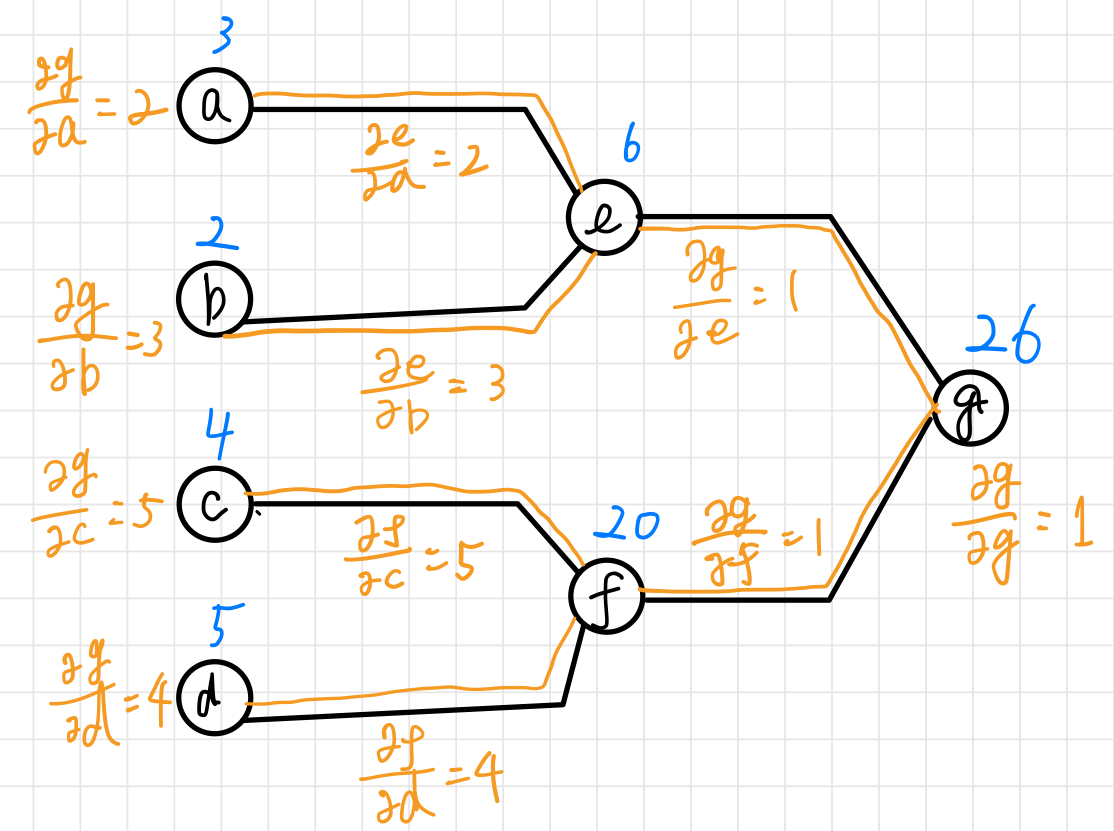
\includegraphics[width=8cm]{./capture/calc_graph.png}
  \caption{計算グラフ}
  \label{fig:calc_graph}
\end{figure}

\begin{figure}[htbp]
  \centering
  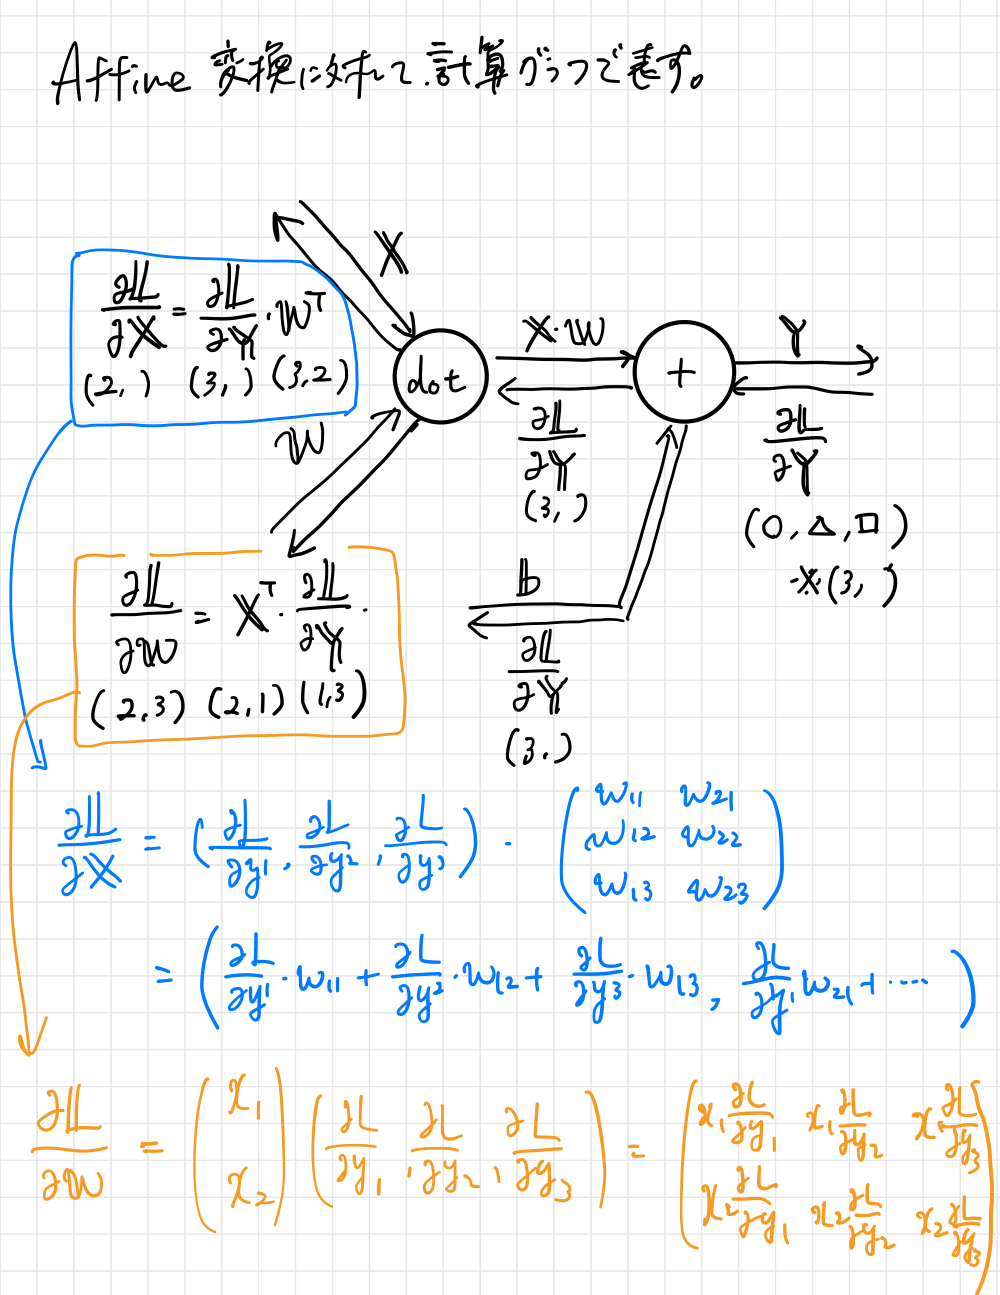
\includegraphics[width=8cm]{./capture/affine_calc_graph.png}
  \caption{Affine変換を計算グラフで表す}
  \label{fig:affine_calc_graph}
\end{figure}
  
\newpage

\paragraph{参考文献}
\begin{enumerate}
  \item 岡谷貴之/深層学習 改訂第2版 [機械学習プロフェッショナルシリーズ]/ 講談社サイエンティフィク/ 2022-01-17
  \item DeepLearning- 計算グラフについて理解する/@edo\_m18(Kazuya Hiruma) \url{https://qiita.com/edo_m18/items/7c95593ed5844b5a0c3b}
  \item 誤差逆伝播法を計算グラフを使って分かりやすく解説する \url{https://deepage.net/deep\_learning/2017/04/02/backpropagation.html}
  \item 交差エントロピー誤差をわかりやすく説明してみる/@kenta1984(Kenta Sasaki) \url{https://qiita.com/kenta1984/items/59a9ef1788e6934fd962}
\end{enumerate}


\end{document}